\section{算法设计}\label{algorithm}
\subsection{系统框架}
本文的系统框架如图\ref{system}所示。该系统以一系列连续的点云帧作为输入,相较于其他使用RGB-D图像作为输入的系统,无需使用相机姿态与内参。该系统维护了两个独立的线程:使用输入数据进行逐帧建图和进行关键帧选择的增量建图线程;在关键帧集合中选择优化对象进行批量训练,以对全局地图进行优化的全局建图线程。

当系统启动时,增量建图线程加载数据,根据每一帧中的点云分配体素和初始化特征。在随后进行的可微渲染过程中,生成采样光线并使用真实数据对地图特征与解码器进行监督训练。在增量线程中使用了一个关键帧选择策略,将符合条件的点云帧放入关键帧集合。全局建图线程维护一个关键帧窗口,对被随机选中的关键帧同步的进行批量采样和渲染,进而对地图进行全局的优化。两个线程共享的数据包括关键帧集合,被嵌入特征的体素网格和解码器参数。
\begin{figure}[htbp]
    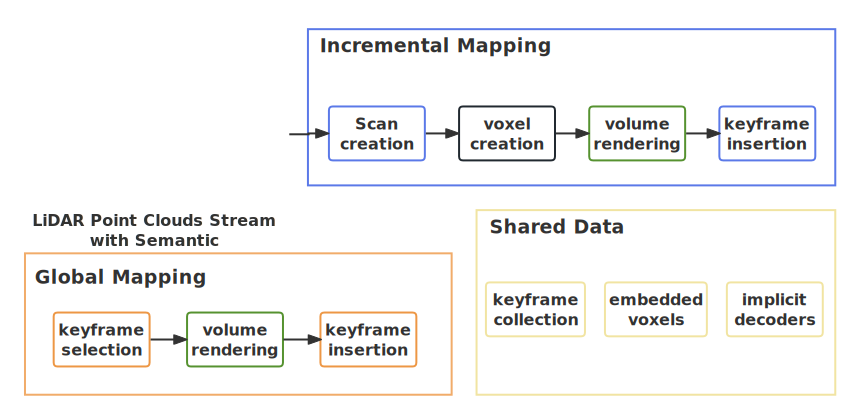
\includegraphics[scale = 0.355]{figures/system.jpg}
    \centering
    \caption{系统概览。该系统维护了两个独立的线程,以带语义的点云作为输入,分别对地图进行增量建图与全局建图。两者共享了包括地图特征在内的资源数据,同步的对地图进行优化。}\label{system}
\end{figure}
\subsection{基于点云的体渲染}
本文使用点云数据进行监督训练,将每一次激光雷达扫描(Scan)的结果作为一帧$f$,因此整个系统输入的数据为一系列连续的点云帧。每一帧包含一个激光雷达3D坐标$\mathbf{x}\in \mathbb{R}^3 $与一个点云集合$P$。其中每一个点云$p\in P$都包含其自身的3D坐标$\mathbf{x}_p\in \mathbb{R}^3$与一个语义标签索引$s\in \mathbb{R}$。
\subsubsection{体素采样}
本文使用一个隐式的SDF解码器$F_\theta$,一个隐式的语义解码器$G_\phi$(其中$\theta$和$\phi$为可优化的网络参数)和一个$N$维的存储在稀疏体素中的特征集合来表示一个场景。这些特征存储在每一个体素的8个顶点上,每一个特征都被相邻的体素共享,这些共享的特征可以优化体素边界上出现的伪影。

由于本文的体素是动态分配的,对于尚未进行建图的区域空间中存在大量的空白体素。因此,在空间中进行分层随机采样的方法会在无效的体素上浪费大量的运算资源。为了提高采样效率,对于当前点云帧中每一个被采样的点云,本文首先通过一个求交运算,检查这条沿着从雷达位置到该点的光线是否穿过了任何有效体素。没有击中任何体素的采样点云会被剔除,因为其不会对渲染产生任何影响。考虑到复杂的大规模场景可能存在较远的边界,本文设置了一个采样点所能影响到的体素的最大数量$M_h$和最大的采样距离$D_{max}$。

如图\ref{shinemapping}所示,对于模拟出的光线,本文将以固定步长在从雷达位置到最大采样距离的有效体素上进行等距采样。对于光线上的任意一个采样点,本文使用其处于的叶子节点上的8个$N$维特征进行三线性插值,得出该点的特征值。随后使用解码器进行解码。
\begin{figure}[htbp]
    \includegraphics[scale = 0.3]{figures/shinemapping.png}
    \centering
    \caption{一次迭代中的正向传播步骤:首先模拟一条从激光雷达处发出的穿过被采样点云的光线,随后在光线上以固定步长采样(a),对于空间中每一个采样点,对叶子节点体素使用三线性插值计算出特征值(b),最后使用SDF解码器与语义解码器计算出最终结果(c)。}\label{shinemapping}
\end{figure}
\subsubsection{解码器}
如图\ref{shinemapping}所示,本文使用两个较浅的全连接层(MLP)$F_\theta$和$G_\phi$分别用来预测空间中任意一点的SDF值与语义信息。其中$F_\theta$的输出为一个SDF数值,代表该点距离最近表面的距离;$G_\phi$的输出为一个$N_{sem}$维向量,其中$N_{sem}$表示语义标签种类的个数。该向量在推理时会被执行一次argmax函数得到最终语义标签的索引。
\subsubsection{隐式表面渲染}
相较于原始NeRF中使用MLP预测空间中任意一点的体密度,也就是占据概率, SDF能更好的表达几何信息,这也是为什么可以将其用于光线追踪中等任务中,因此本文在训练中直接回归SDF值。下列渲染公式表示了如何从嵌套在体素中的特征中获得该处点云最终的深度$D$和语义向量$\mathbf{S}$。假设在一条光线上采样$N$个点:
\begin{equation}
\begin{alignedat}{2}
    &s_i&&=F_\theta(\mbox{TriLerp}(T_i\mathbf{p}_i,\mathbf{e}))\;,\\
    &\mathbf{S}_i&&=G_\phi(\mbox{TriLerp}(T_i\mathbf{p}_i,\mathbf{e}))\;,\\
    &w_i&&=\mathbf{\sigma}(\frac{s_i}{tr})\cdot\mathbf{\sigma}(-\frac{s_i}{tr})\;,\\
    &\mathbf{S} &&= \frac{1}{\sum_{j=0}^{N-1}w_j}\sum_{i=0}^{N-1}w_i\cdot\mathbf{S}_i\;,\\
    &D &&= \frac{1}{\sum_{j=0}^{N-1}w_j}\sum_{i=0}^{N-1}w_i\cdot d_i
\end{alignedat}
\end{equation}
其中$T_i$表示当前帧激光雷达的位置, $\mathbf{p}_i$表示该点在体素中的相对坐标,$\mbox{TriLerp}(\cdot , \cdot)$表示三线性插值函数, $\mathbf{e}$表示存储在体素中的特征。$F_\theta\mbox{和}G_\phi$分别为带可优化网络参数的解码器。为了计算每一个采样点的权重$w_i$, 本文使用sigmoid函数$\mathbf{\sigma}$计算sdf值$s_i$与先前设置的截断距离$tr$的比值。本文使用该权重对这条光线上的每个采样点的语义向量$\mathbf{S}_i$进行加权积分得到最终结果$\mathbf{S}$。同样的,为了得到深度值,本文对这条光线上每一个采样点的深度进行积分,其中$d_i$为第$i$个采样点的深度。
\subsection{建图}
\subsubsection{地图优化}
为了监督网络训练,本文尝试了多种损失函数,分别为semantic loss, depth loss, free-space loss, SDF loss和二元交叉熵BCE loss。其中semantic loss为多元交叉熵函数,depth loss为L1损失函数。给定采样点云集合$P$:
\begin{equation}
\begin{alignedat}{2}
    &\mathcal{L}_{sem} &&= -\frac{1}{|P|}\sum_{i=0}^{|P|}\sum_{j=0}^{N_{sum}}\mathbf{S}_i^{gt}[j]\log(\mathbf{S}_i[j])\;,\\
    &\mathcal{L}_{depth} &&= \frac{1}{|P|}\sum_{i=0}^{|P|}\| D_i-D_i^{gt}\Vert\;,
\end{alignedat}
\end{equation}
其中$\mathbf{S}_i$和$D_i$为点云帧集合中第$i$个点渲染出的语义向量和深度,与之对应的$\mathbf{S}_i^{gt}$同样为$N_{sem}$维向量,除语义标签索引位置为1之外其余位置均为0, $\mathbf{S}_i[j]$表示其中的第$j$个元素; $D_i^{gt}$为该帧中激光雷达到该点的欧式距离。 

在基于SDF的建图中,需要被关注应该是其SDF值为0的点,因为这些点定义了表面。因此,越接近采样点云的采样点应该对最终SDF值的作用更大,反之,离点云越远的点其作用也更小。本文分别使用了SHINE-Mapping中的二元交叉熵损失函数和Vox-Fusion中的free-space loss和sdf loss两个L2损失函数。

SDF二元交叉熵函数的计算过程为,首先通过带超参数$\sigma$的sigmoid函数$S(x) = 1/(1 + e^{x/\sigma})$,其中超参数$\sigma$用来控制函数的平滑度,将sdf值映射到$[0,1]$区间上。给定一个采样点$\mathbf{x}_i\in \mathbb{R}^3$,计算其投影至表面(假设每个被采样的点云均在表面上)的距离$d_i$,使用经过映射后的值$l_i=S(d_i)$作为监督值。之后应用二元交叉熵作为本文的损失函数:
\begin{equation}
    \mathcal{L}_{bce} = l_i\cdot \log(o_i)+(1-l_i)\cdot\log(1-o_i),\label{bce}
\end{equation}
其中$o_i=S(F_\theta(\mbox{TriLerp}(T_i\mathbf{p}_i,\mathbf{e})))$,即经过映射后的渲染出的SDF值。
free-space loss是为了使解码器学习截断距离$tr$,尤其是位于采样点表面附近的符号为正的截断区域内的截断值,然后使用sdf loss在截断区域内学习SDF值以此来使解码器精确的表示表面。本文在渲染时将SDF值为$-tr$的点剔除。
\begin{equation}
    \begin{alignedat}{2}
        &\mathcal{L}_{fs} &&= \frac{1}{|P|}\sum_{p\in P}\frac{1}{S_p^{fs}}\sum_{s\in S_p^{fs}}(D_s-tr)^2,\\
    &\mathcal{L}_{sdf} &&= \frac{1}{|P|}\sum_{p\in P}\frac{1}{S_p^{tr}}\sum_{s\in S_p^{tr}}(D_s-D_s^{gt})^2.\label{voxloss}
    \end{alignedat}
\end{equation}
本文在优化时对地图特征与解码器均应用了ADAM\cite{adam}优化方法,最终的损失函数为:
\begin{equation}
    \mathcal{L} = \lambda_{sem}\mathcal{L}_{sem}+\lambda_{depth}\mathcal{L}_{depth}+\lambda_{bce}\mathcal{L}_{bce}+\lambda_{fs}\mathcal{L}_{fs}+\lambda_{sdf}\mathcal{L}_{sdf}
\end{equation}
其中$\lambda$表示不同损失函数的权重。在实际情况中,对于SDF的监督通常只使用式\ref{bce}或式\ref{voxloss}中的一种损失函数。
\subsubsection{动态体素管理}
相较于在运行前就将整个场景编码,本文只关注已经被观察到的场景表面,因此使用动态体素管理方法进行体素的分配与搜索。本文将整个场景使用八叉树进行切分为互不包含的体素。这些体素与坐标轴平行,作为组成场景的元素和八叉树的叶子节点。

首先将尚未观察到的场景区域的叶子节点初始化为空,当新的一帧进入系统时,将该帧中的所有点云变化至世界坐标系。如果这些点云落在了尚未分配的体素中,系统将为这些点云分配新的体素。由于本文设置了八叉树的最大层树$L_{max}$,因此每个点云会被放置在最小的叶子节点中。该过程不需要采样,而是对所有点进行计算,因此使用八叉树结构可以更快的进行分配和索引。
\subsubsection{全局建图与关键帧选择}\label{forgettingsection}
\begin{figure}[htbp]
    \includegraphics[scale = 0.2]{figures/forgetting.jpg}
    \centering
    \caption{在特征网格中进行增量建图时发生遗忘问题的例子,图源SHINE-Mapping\cite{shine}} \label{forgetting}
\end{figure}
将大规模场景以增量建图方法编码会受到灾难性遗忘(Catastrophic Forgetting)问题的限制。如图\ref{forgetting}所示,在每一帧中($T_0, T_1$和$T_2$),系统仅能观察到环境的部分信息。在增量建图中的第$T_0$帧,使用从区域A0获取到的信息优化存储在网格中的特征$V_0, V_1, V_2$和$V_3$,因此$V_0, V_1, V_2$和$V_3$这4个特征将能较精确的表示区域A0的几何信息。然而当相机向前移动,使用T1帧更新$V_0, V_1, V_2$和$V_3$的特征时,网络将仅关注生成$A_1$时的损失,不再关注$A_0$区域的表现。当相机进一步移动至$T_2$帧时,$V_2$和$V_3$中的特征将再次被更新,但网络无法保证不会影响到$A_0$和$A_1$区域的建图精度。这就是遗忘问题发生的原因。

为了解决灾难性遗忘问题,本文记录关键帧对网络进行重复训练。系统维护了一个关键帧集合K,使用Vox-Fusion中的策略,即八叉树体素结构的变化量决定何时插入关键帧:每当新的一帧出现时,体素管理系统会执行求交运算得出需要新分配体素的数量$N_c$,而当前存储的体素数量为$N_o$,当两者比值$p_{kf}=N_c/N_o$大于某一阈值时,当前帧将被插入关键帧集合。某种极端情况下,当相机移动处于一个循环状态时,可能出现只有极少体素或没有体素被新分配,导致永远没有关键帧被插入。因此,本文也设定了相邻关键帧的最大距离,例如,当之前的$N$帧都不是关键帧时,自动插入一个关键帧。

在第全局建图线程中,本文使用一个大小为$N_{kf}$的窗口从关键帧集合$K$中随机选取$N_{kf}$个关键帧,与当前帧一起,共$N_{kf}+1$帧作为优化目标对地图进行全局优化,与增量建图线程同步进行。在增量建图结束后,使用全局建图线程随机选择优化目标对整个地图执行$N_f$次迭代训练,完成最后的建图优化。
